\documentclass{article}

\title{Gravity Lab}
\author{Henry Oehlrich \and Grace Jiang \and Ansh Aggrawal}

\usepackage{tikz}
\usepackage{capt-of}
\usepackage[labelfont=bf]{caption}
\usepackage[margin=1.25in]{geometry}
\usepackage{booktabs}
\usepackage{array}
\usepackage{siunitx}
\usepackage{amsmath}
\usepackage{csvsimple}
\usepackage{pgfplots}
\usepackage{pgfplotstable}

\pgfplotsset{compat=1.18}
\newcolumntype{L}{>{$}l<{$}}

\begin{document}
\maketitle

\begin{figure}[ht]
    \begin{minipage}[b]{0.5\textwidth}
        \centering
        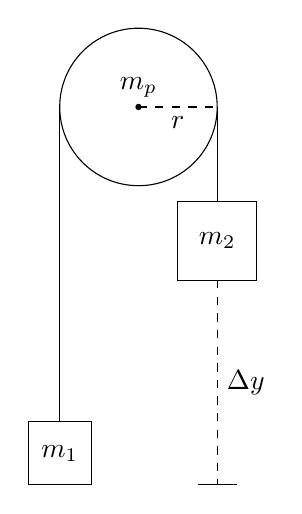
\begin{tikzpicture}
            \draw (0,5) node[above] {$m_p$} circle (1);
            \fill (0,5) circle (0.04);
            \draw[dashed] (0,5) -- (0.5, 5) node[below] {$r$} -- (1,5);

            \draw (1,5) -- (1,3.8);
            \draw (0.5,3.8) rectangle node {$m_2$} ++(1,-1);

            \draw (-1,5) -- (-1,1);
            \draw (-1.4,1) rectangle node {$m_1$} ++(0.8,-0.8);

            \draw[dashed] (1,2.8) -- (1,1.5) node[right] {$\Delta y$} -- (1,0.2);
            \draw (0.75,0.2) -- (1.25,0.2);
        \end{tikzpicture}
        \caption{Lab setup}
        \label{fig:setup}
    \end{minipage}%
    \begin{minipage}[b]{0.5\textwidth}
        \centering
        \begin{tabular}{l|l}
            \toprule
            Symbol & Value \\
            \midrule
            $\Delta y$ & \qty{1.70}{\meter} \\
            $m_1$ & \qty{0.01}{\kilogram} \\
            $g$ & \qty{9.81}{\meter\per\second\squared} \\
            $m_p$ & \qty{0.05}{\kilogram} \\
            $r$ & \qty{0.05}{\meter} \\
            $m_2$ & varied \\
            $t$ & measured \\
        \end{tabular}
        \captionof{table}{Constants and Variables}
    \end{minipage}
\end{figure}

\begin{equation}
    F_s = g(m_2 - m_1)
\end{equation}

\begin{figure}[ht]
    \begin{minipage}[b]{0.5\textwidth}
        \centering
        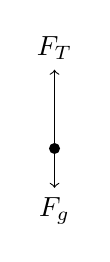
\begin{tikzpicture}
            \fill (0,0) circle (0.07);
            \draw[->] (0,0) -- (0,-0.5) node[below] {$F_g$};
            \draw[->] (0,0) -- (0,1) node[above] {$F_T$};
        \end{tikzpicture}
        \caption{Free body diagram of $m_1$}
        \label{fig:fbd1}
    \end{minipage}%
    \begin{minipage}[b]{0.5\textwidth}
        \centering
        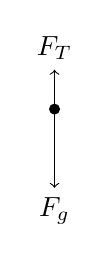
\begin{tikzpicture}
            \fill (0,0) circle (0.07);
            \draw[->] (0,0) -- (0,-1) node[below] {$F_g$};
            \draw[->] (0,0) -- (0,0.5) node[above] {$F_T$};
        \end{tikzpicture}
        \caption{Free body diagram of $m_2$}
        \label{fig:fbd2}
    \end{minipage}%
\end{figure}

\begin{figure}[ht]
    \centering
    \begin{tabular}{l|l|l|l}
        \toprule
        $m_2$ (\si{\kilogram}) & time (\si{\second}) & $m_2 - m_1$ (\si{\kilogram}) & $F_s$ (\si{\newton}) \\
        \midrule
        0.02 & 1.461 & 0.01 & 0.0478 \\
        0.02 & 1.441 & 0.01 & 0.0491 \\
        0.02 & 1.228 & 0.01 & 0.0676 \\
        0.02 & 1.195 & 0.01 & 0.0714 \\
        0.02 & 1.276 & 0.01 & 0.0626 \\
        0.02 & 1.290 & 0.01 & 0.0613 \\
        0.02 & 1.860 & 0.01 & 0.0295 \\
        0.03 & 0.936 & 0.02 & 0.155 \\
        0.03 & 1.016 & 0.02 & 0.132 \\
        0.03 & 0.949 & 0.02 & 0.151 \\
        0.03 & 1.009 & 0.02 & 0.134 \\
        0.03 & 1.006 & 0.02 & 0.134 \\
        0.03 & 0.931 & 0.02 & 0.157 \\
        0.03 & 1.000 & 0.02 & 0.136 \\
        0.10 & 0.667 & 0.09 & 0.840 \\
        0.10 & 0.683 & 0.09 & 0.802 \\
        0.10 & 0.669 & 0.09 & 0.835 \\
        0.10 & 0.686 & 0.09 & 0.795 \\
        0.10 & 0.691 & 0.09 & 0.783 \\
        0.04 & 0.896 & 0.03 & 0.212 \\
        0.04 & 0.823 & 0.03 & 0.251 \\
        0.04 & 0.801 & 0.03 & 0.265 \\
        0.04 & 0.897 & 0.03 & 0.211 \\
        0.04 & 0.834 & 0.03 & 0.244 \\
        0.04 & 0.887 & 0.03 & 0.216 \\
        0.04 & 0.889 & 0.03 & 0.210 \\
        0.05 & 0.763 & 0.04 & 0.350 \\
        0.05 & 0.798 & 0.04 & 0.320 \\
        0.05 & 0.789 & 0.04 & 0.328 \\
        0.05 & 0.795 & 0.04 & 0.323 \\
        0.05 & 0.807 & 0.04 & 0.313 \\
        0.05 & 0.781 & 0.04 & 0.334 \\
    \end{tabular}
    \caption{Data}
    \label{fig:data}
\end{figure}

\begin{figure}
    \centering
    \begin{tikzpicture}
        \begin{axis}[
                xlabel={$m_2 - m_1$ (\si{\kilogram})},
                ylabel={$F_s$ (\si{\newton})},
                xmin=0,xmax=0.1,
                ymin=0,ymax=1.1,
                tick label style={/pgf/number format/fixed},
                scaled ticks=false,
                width=0.7\textwidth,
            ]
            \addplot +[only marks,mark size=1.5pt] table
                {xy.dat};
            \addplot table [
                y={create col/linear regression={y=force}},
                mark=none,
            ]
                {xy.dat};
            \addlegendentry{$F_s = a_s(m_2+m_1)$}
            \addlegendentry{$\hat{F_s} = \pgfmathprintnumber{\pgfplotstableregressiona}(m_2-m_1)$}
            \addlegendentry{$F_s = g(m_2-m_1)$}
        \end{axis}
    \end{tikzpicture}
    \caption{Scatterplot of Linearized Data}
    \label{fig:scatterxy}
\end{figure}

\begin{figure}
    \centering
    \begin{tikzpicture}
        \begin{axis}[
                xlabel={$m_2 - m_1$ (\si{\kilogram})},
                ylabel={Residual (\si{\newton})},
                xmin=0,xmax=0.1,
                ymin=-0.04,ymax=0.04,
                tick label style={/pgf/number format/fixed},
                scaled ticks=false,
                width=0.7\textwidth,
            ]
            \draw[dashed] (0,0) -- (1,0);
            \addplot +[only marks,mark size=1.5pt] table
                {residual.dat};
        \end{axis}
    \end{tikzpicture}
    \caption{Residual Plot}
    \label{fig:residual}
\end{figure}


\end{document}
